\chapter{Architectural Design}
\section{Overview: high-level components and interactions}
This section provides an overview of the system's architectural components and their interactions.

\begin{figure}[h]
    \centering
    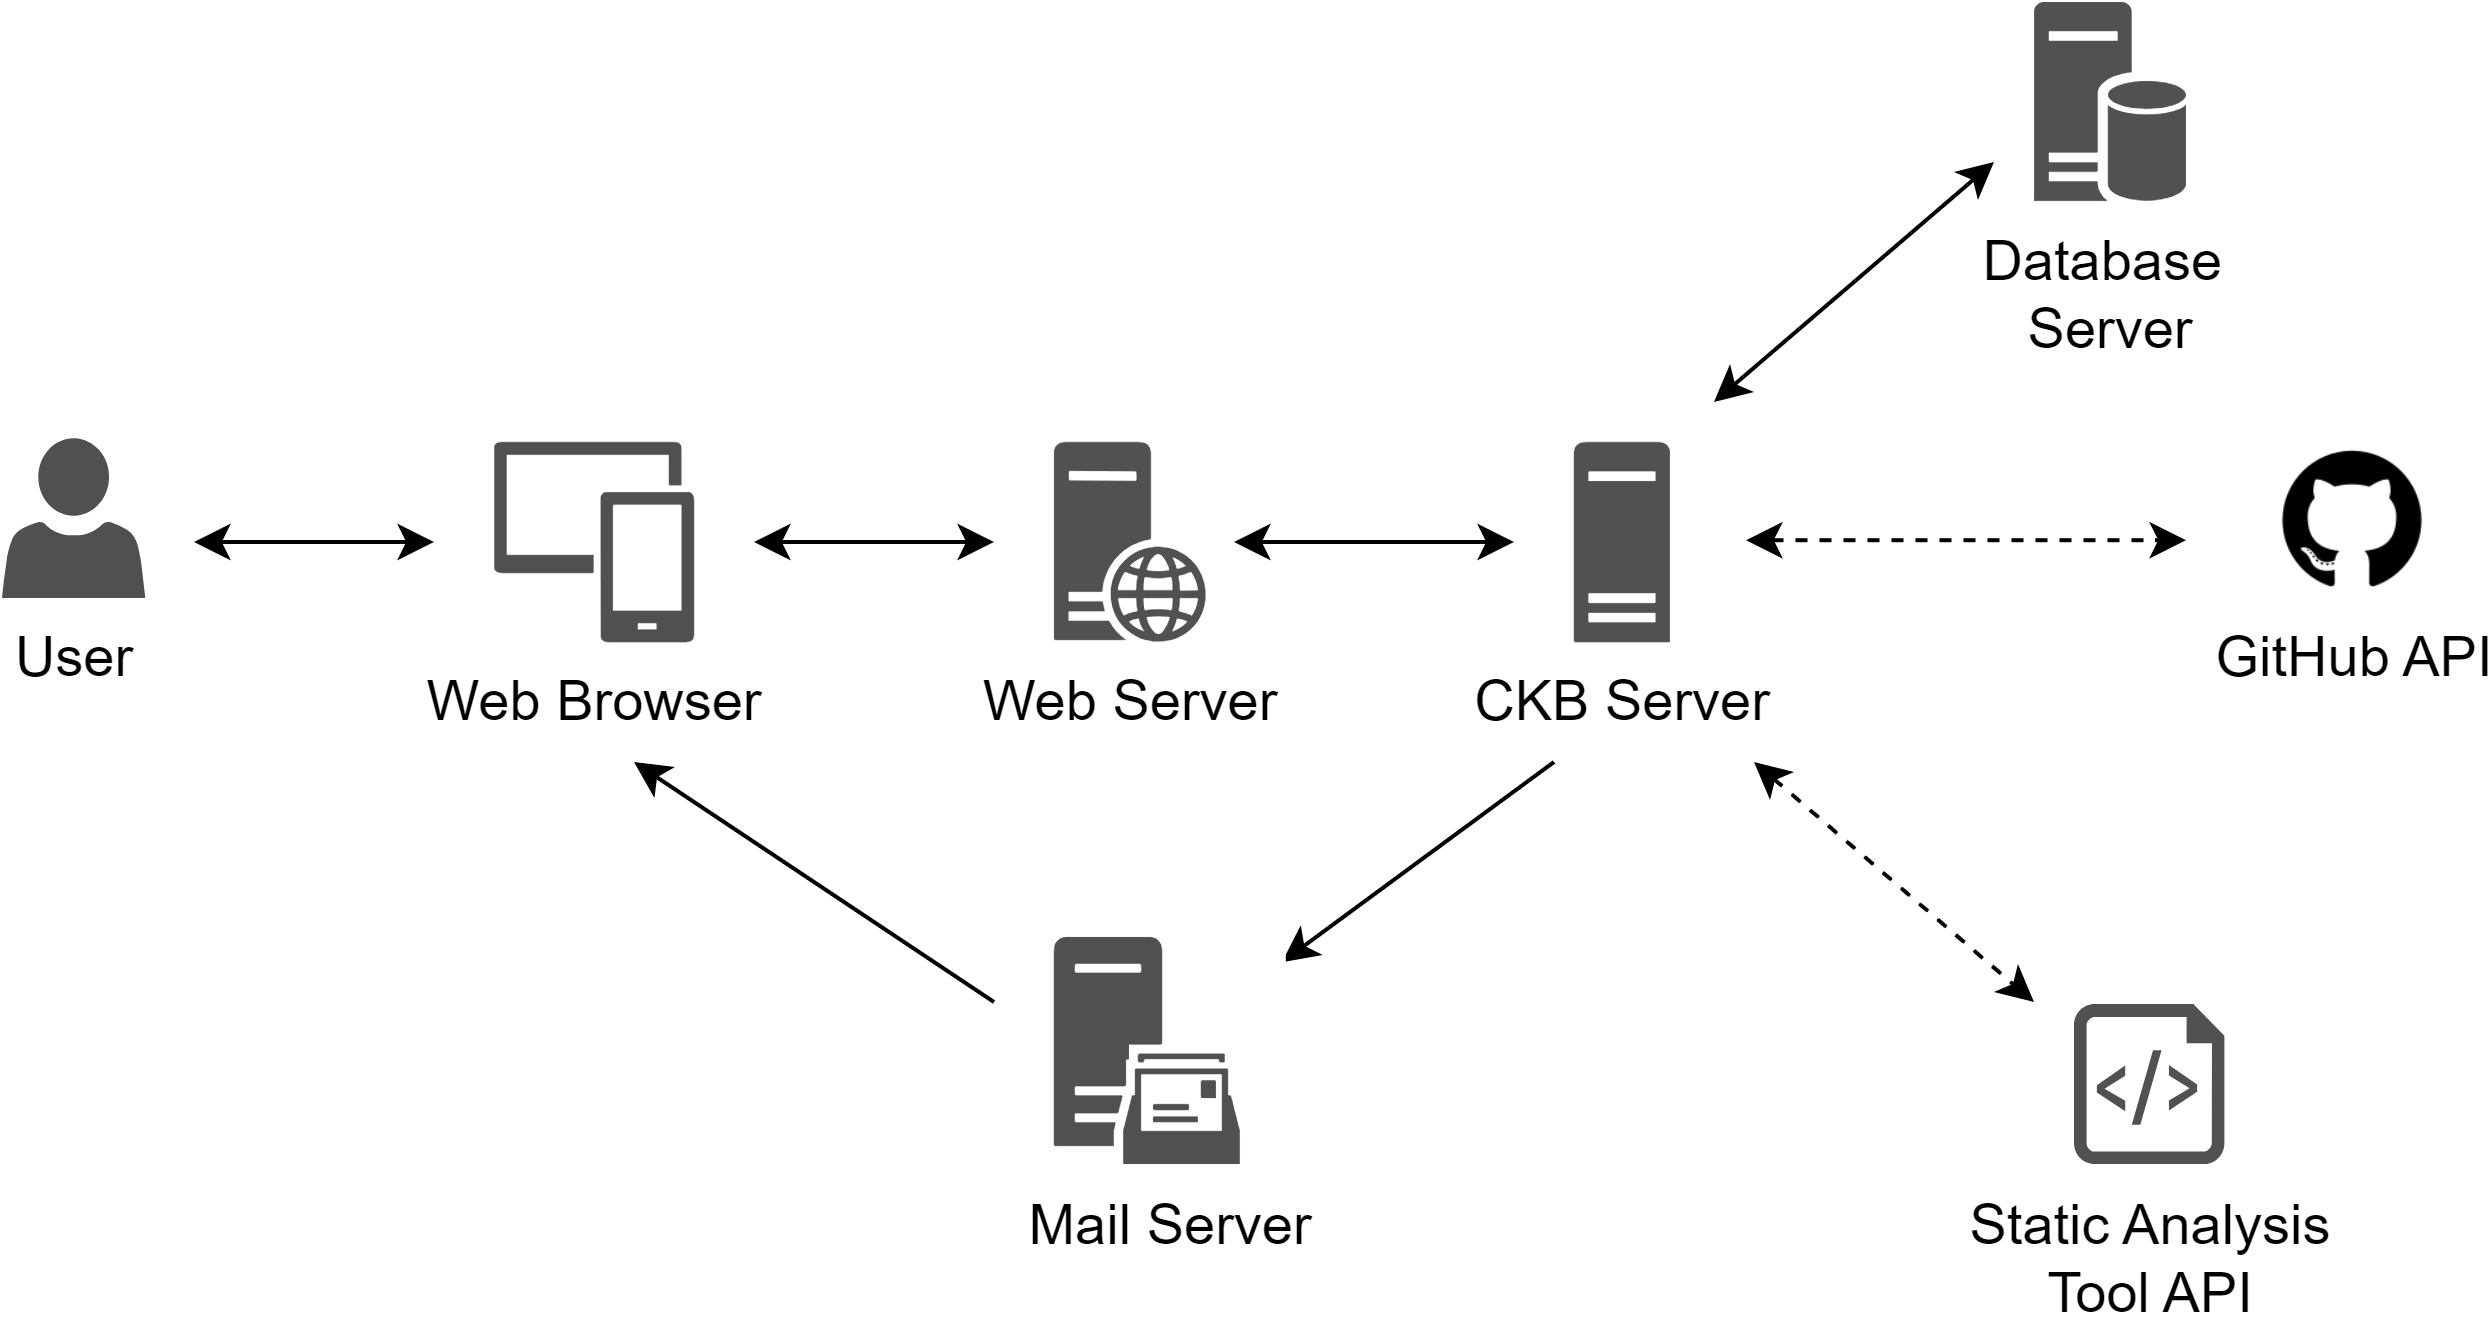
\includegraphics[scale=0.5]{images/hl-system.png}
    \caption{CKB system overview}
    \label{fig:CKBoverview}
\end{figure}

The CKB system will be developed using the client-server paradigm:
\begin{itemize}
    \item Server side:
    \begin{itemize}
        \item Web Server: used to communicate with web browsers.
        \item CKB Server: where all the logic is located. It communicates with all other server and external tool and API. It is the central point of the system.
        \item Database Server: where all information are located.
        \item Mail Server: used to send all notifications to the users.
        \item GitHub API: used by the system to detect new push in the forked repository of the battles.
        \item Static analysis tool: used by the system to retrieve the quality level of the student's sources, in order to perform the automatic evaluation. 
    \end{itemize}
    \item Client side:
    \begin{itemize}
        \item Web browser: used by all users in order to enter the CKB website.
    \end{itemize}
\end{itemize}

The application will be developed on a three-tiered architecture where the layers (presentation, application, data) are divided into three different tiers. \newline
The client tier is responsible only of the presentation layer, therefore a thin-client has been adopted since the required client-side functionality are limited. The application tier is responsible of the application layer, it receives the request from the clients and handles them. It communicates with the data tier that is responsible of the data layer, it is able to access the data in the database. \newline
Further details on the system components and their interactions will be explained in detail in the following sections.

\section{Component view}
\section{Deployment view}
\section{Component interface}
\section{Run-time view}
\section{Selected architectural styles and patterns}
\subsection*{3-tier Architecture}
\subsection*{Model View Controller Pattern}
\section{Other design decision}